\documentclass[11pt, a4paper]{article}

\usepackage{amsfonts}
\usepackage{amssymb}
\usepackage{amsmath}
\usepackage{epsfig}
\usepackage{graphicx}
\usepackage{tabularx}
\usepackage{parskip}
\usepackage[margin=2.54cm]{geometry}
\usepackage[colorlinks=true]{hyperref}
\usepackage[sort]{natbib}

%%%%%%%%%%%%%%%%%%%%%%%%%%%%%%%%%%%%%%%%%%%%%%%%%%%%%%%%%%%%%%%%%%%%%%%%%%%%%%%%%
%%%%%%%%%%%%%%%%%%%%%%%%%%%%%%%%%%%%%%%%%%%%%%%%%%%%%%%%%%%%%%%%%%%%%%%%%%%%%%%%%
\title{Tag growth}

\author{D'Arcy N. Webber, Jim Thorson}

\date{\today}

\begin{document}
\maketitle

%%%%%%%%%%%%%%%%%%%%%%%%%%%%%%%%%%%%%%%%%%%%%%%%%%%%%%%%%%%%%%%%%%%%%%%%%%%%%%%%%
%%%%%%%%%%%%%%%%%%%%%%%%%%%%%%%%%%%%%%%%%%%%%%%%%%%%%%%%%%%%%%%%%%%%%%%%%%%%%%%%%
%%%%%%%%%%%%%%%%%%%%%%%%%%%%%%%%%%%%%%%%%%%%%%%%%%%%%%%%%%%%%%%%%%%%%%%%%%%%%%%%%
\section{Introduction}
%%%%%%%%%%%%%%%%%%%%%%%%%%%%%%%%%%%%%%%%%%%%%%%%%%%%%%%%%%%%%%%%%%%%%%%%%%%%%%%%%
%%%%%%%%%%%%%%%%%%%%%%%%%%%%%%%%%%%%%%%%%%%%%%%%%%%%%%%%%%%%%%%%%%%%%%%%%%%%%%%%%
%%%%%%%%%%%%%%%%%%%%%%%%%%%%%%%%%%%%%%%%%%%%%%%%%%%%%%%%%%%%%%%%%%%%%%%%%%%%%%%%%
\textit{Dissostichus mawsoni}

Key words: Antarctic toothfish, Ross Sea


%%%%%%%%%%%%%%%%%%%%%%%%%%%%%%%%%%%%%%%%%%%%%%%%%%%%%%%%%%%%%%%%%%%%%%%%%%%%%%%%%
%%%%%%%%%%%%%%%%%%%%%%%%%%%%%%%%%%%%%%%%%%%%%%%%%%%%%%%%%%%%%%%%%%%%%%%%%%%%%%%%%
%%%%%%%%%%%%%%%%%%%%%%%%%%%%%%%%%%%%%%%%%%%%%%%%%%%%%%%%%%%%%%%%%%%%%%%%%%%%%%%%%
\section{Simulation}
%%%%%%%%%%%%%%%%%%%%%%%%%%%%%%%%%%%%%%%%%%%%%%%%%%%%%%%%%%%%%%%%%%%%%%%%%%%%%%%%%
%%%%%%%%%%%%%%%%%%%%%%%%%%%%%%%%%%%%%%%%%%%%%%%%%%%%%%%%%%%%%%%%%%%%%%%%%%%%%%%%%
%%%%%%%%%%%%%%%%%%%%%%%%%%%%%%%%%%%%%%%%%%%%%%%%%%%%%%%%%%%%%%%%%%%%%%%%%%%%%%%%%
Simulated 315 individuals, the same number as in the actual toothfish data
set. The next step was to simulate sex, Age1, Age2 and time at liberty. What I
did in the current simulation run was:
\begin{itemize}
\item Sampled sex from the observed sexes of individuals (with replacement).
\item Sampled Age1, Age2 and time at liberty independently (with replacement)
  from those observed. Randomly selected one of these variables and calculated
  this values given the other two.
\item Rounded Age1, Age2 and time at liberty off to the nearest integer.
\end{itemize}
This is a bit of a hack I know, but the alternative did not yeild realistic
looking Age1, Age2, liberty samples.


I also tried this:
\begin{itemize}
\item Sampled sex using a binomial distribution.
\item Fit lognormal distributions to Age1 and time at liberty and simulate
  independently from the distributions.
\item Calculate Age2 given Age1 and time at liberty.
\item Rounded Age1, Age2 and time at liberty off to the nearest integer.
\end{itemize}
But this resulted in unrealistic Age2's (i.e. when a long time at liberty is
added to an already old fish), the plots just looked a bit silly.

Below are some exmaple plots using the first sampling approach above then
running these through our simulation model. 
\begin{figure}[!htbp]
  \centering
  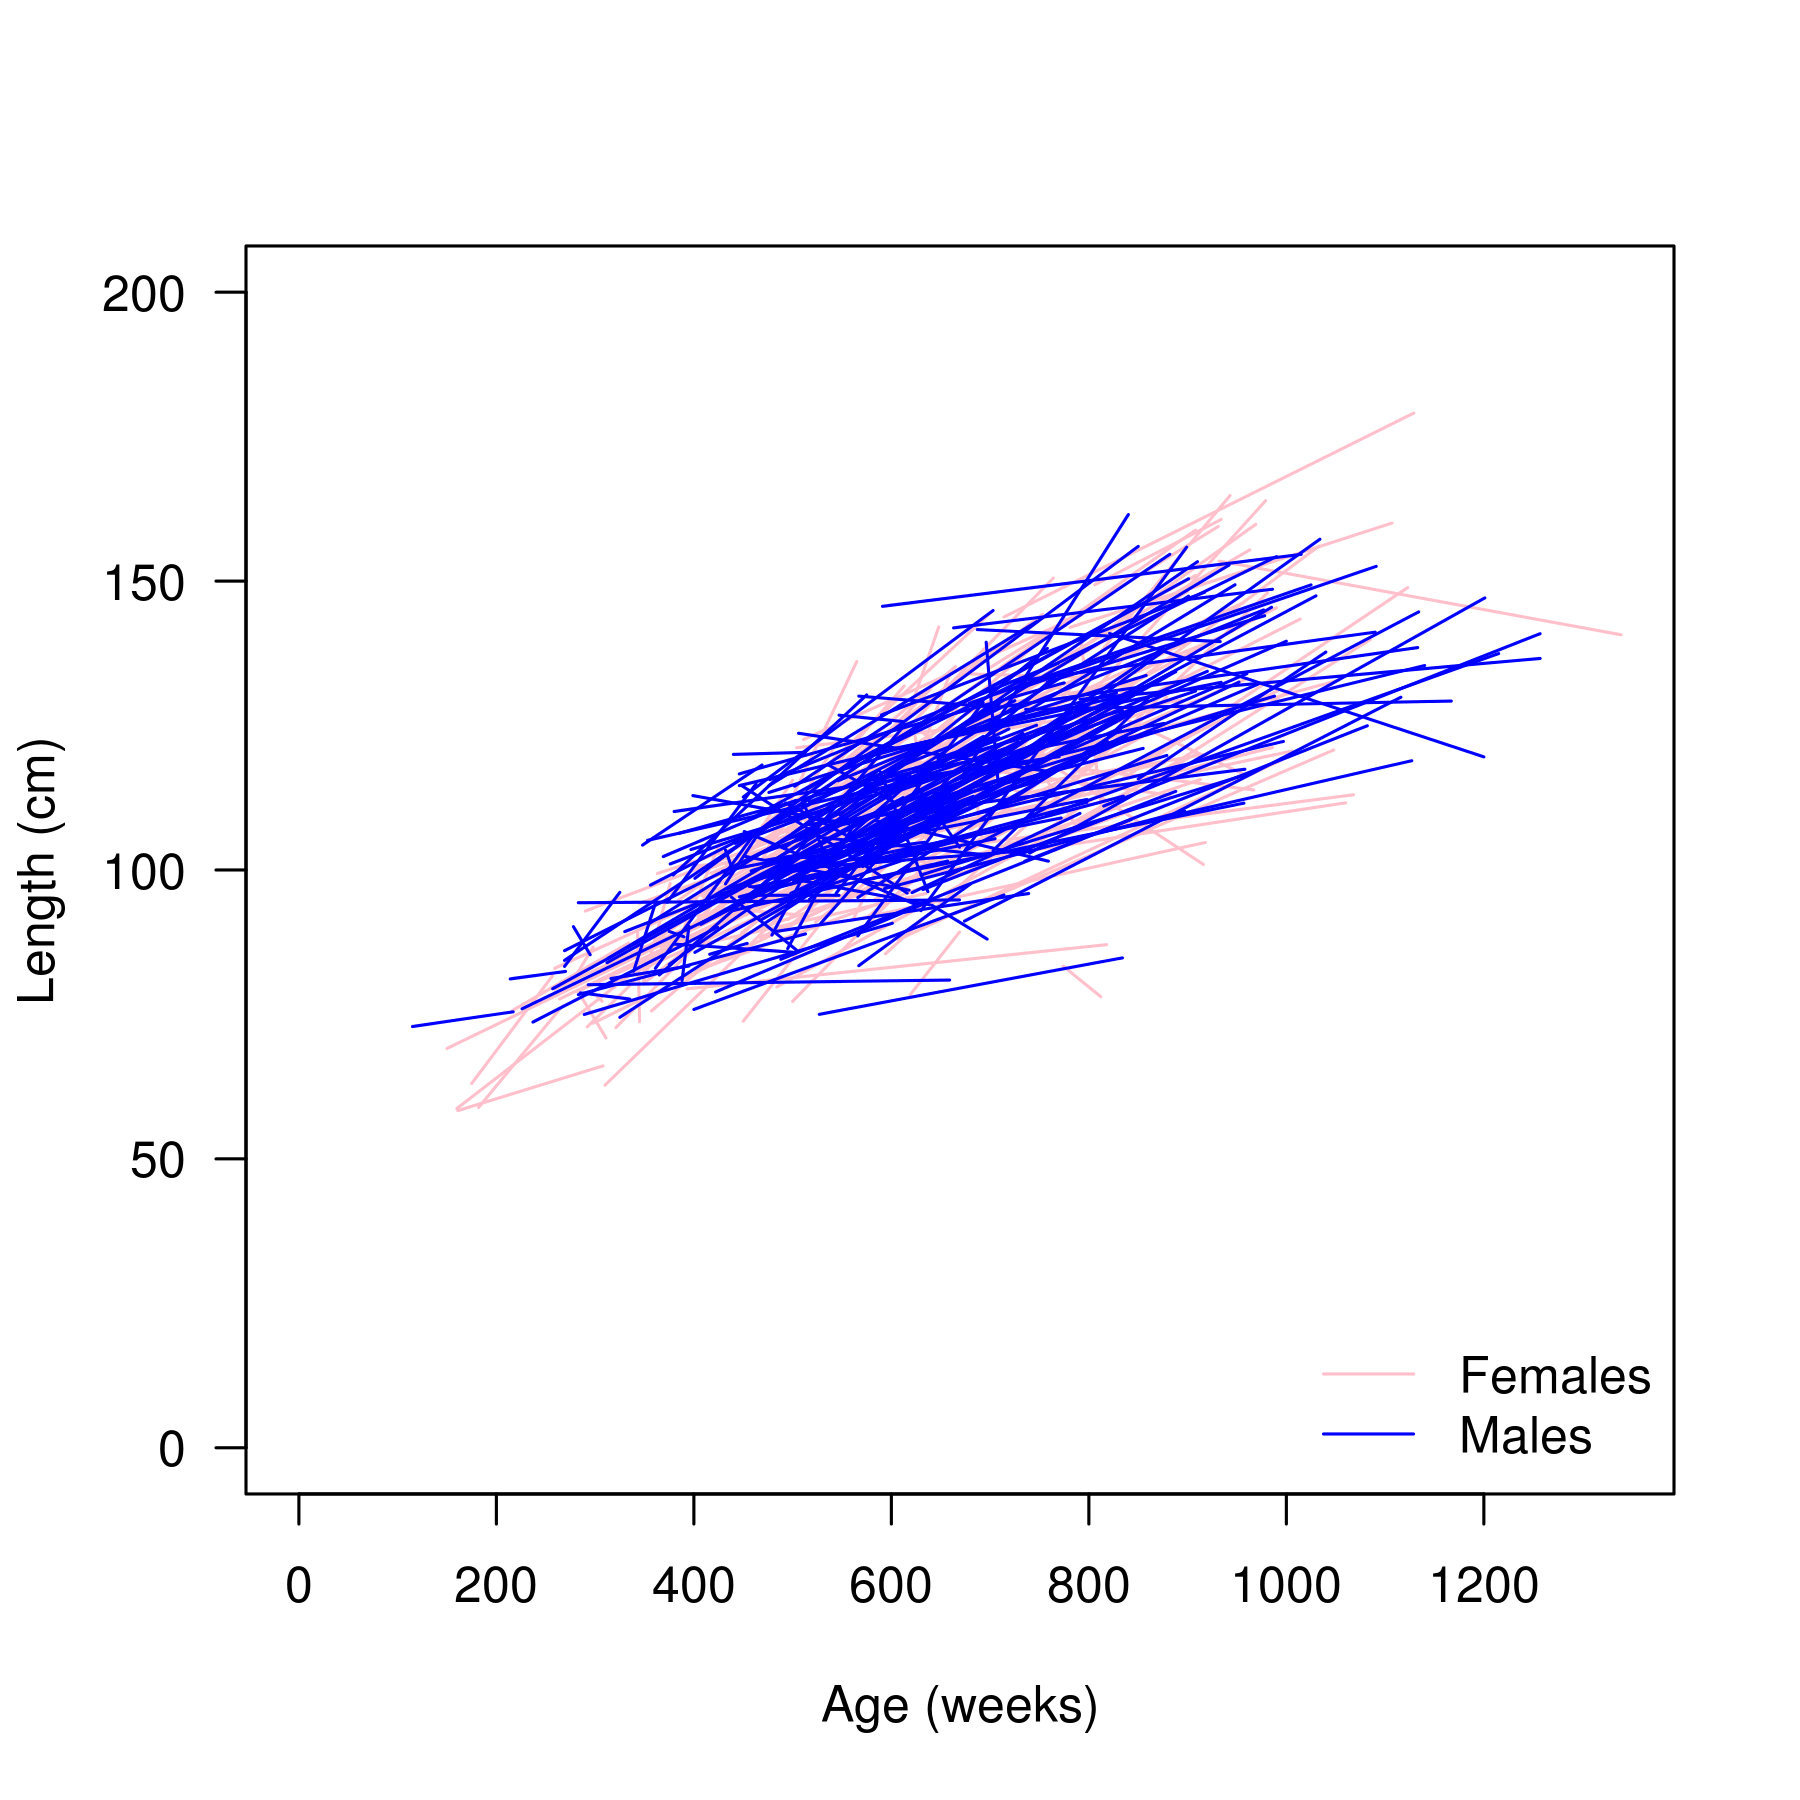
\includegraphics[width=0.49\linewidth]{../simulation/sims/growth-1.png}
  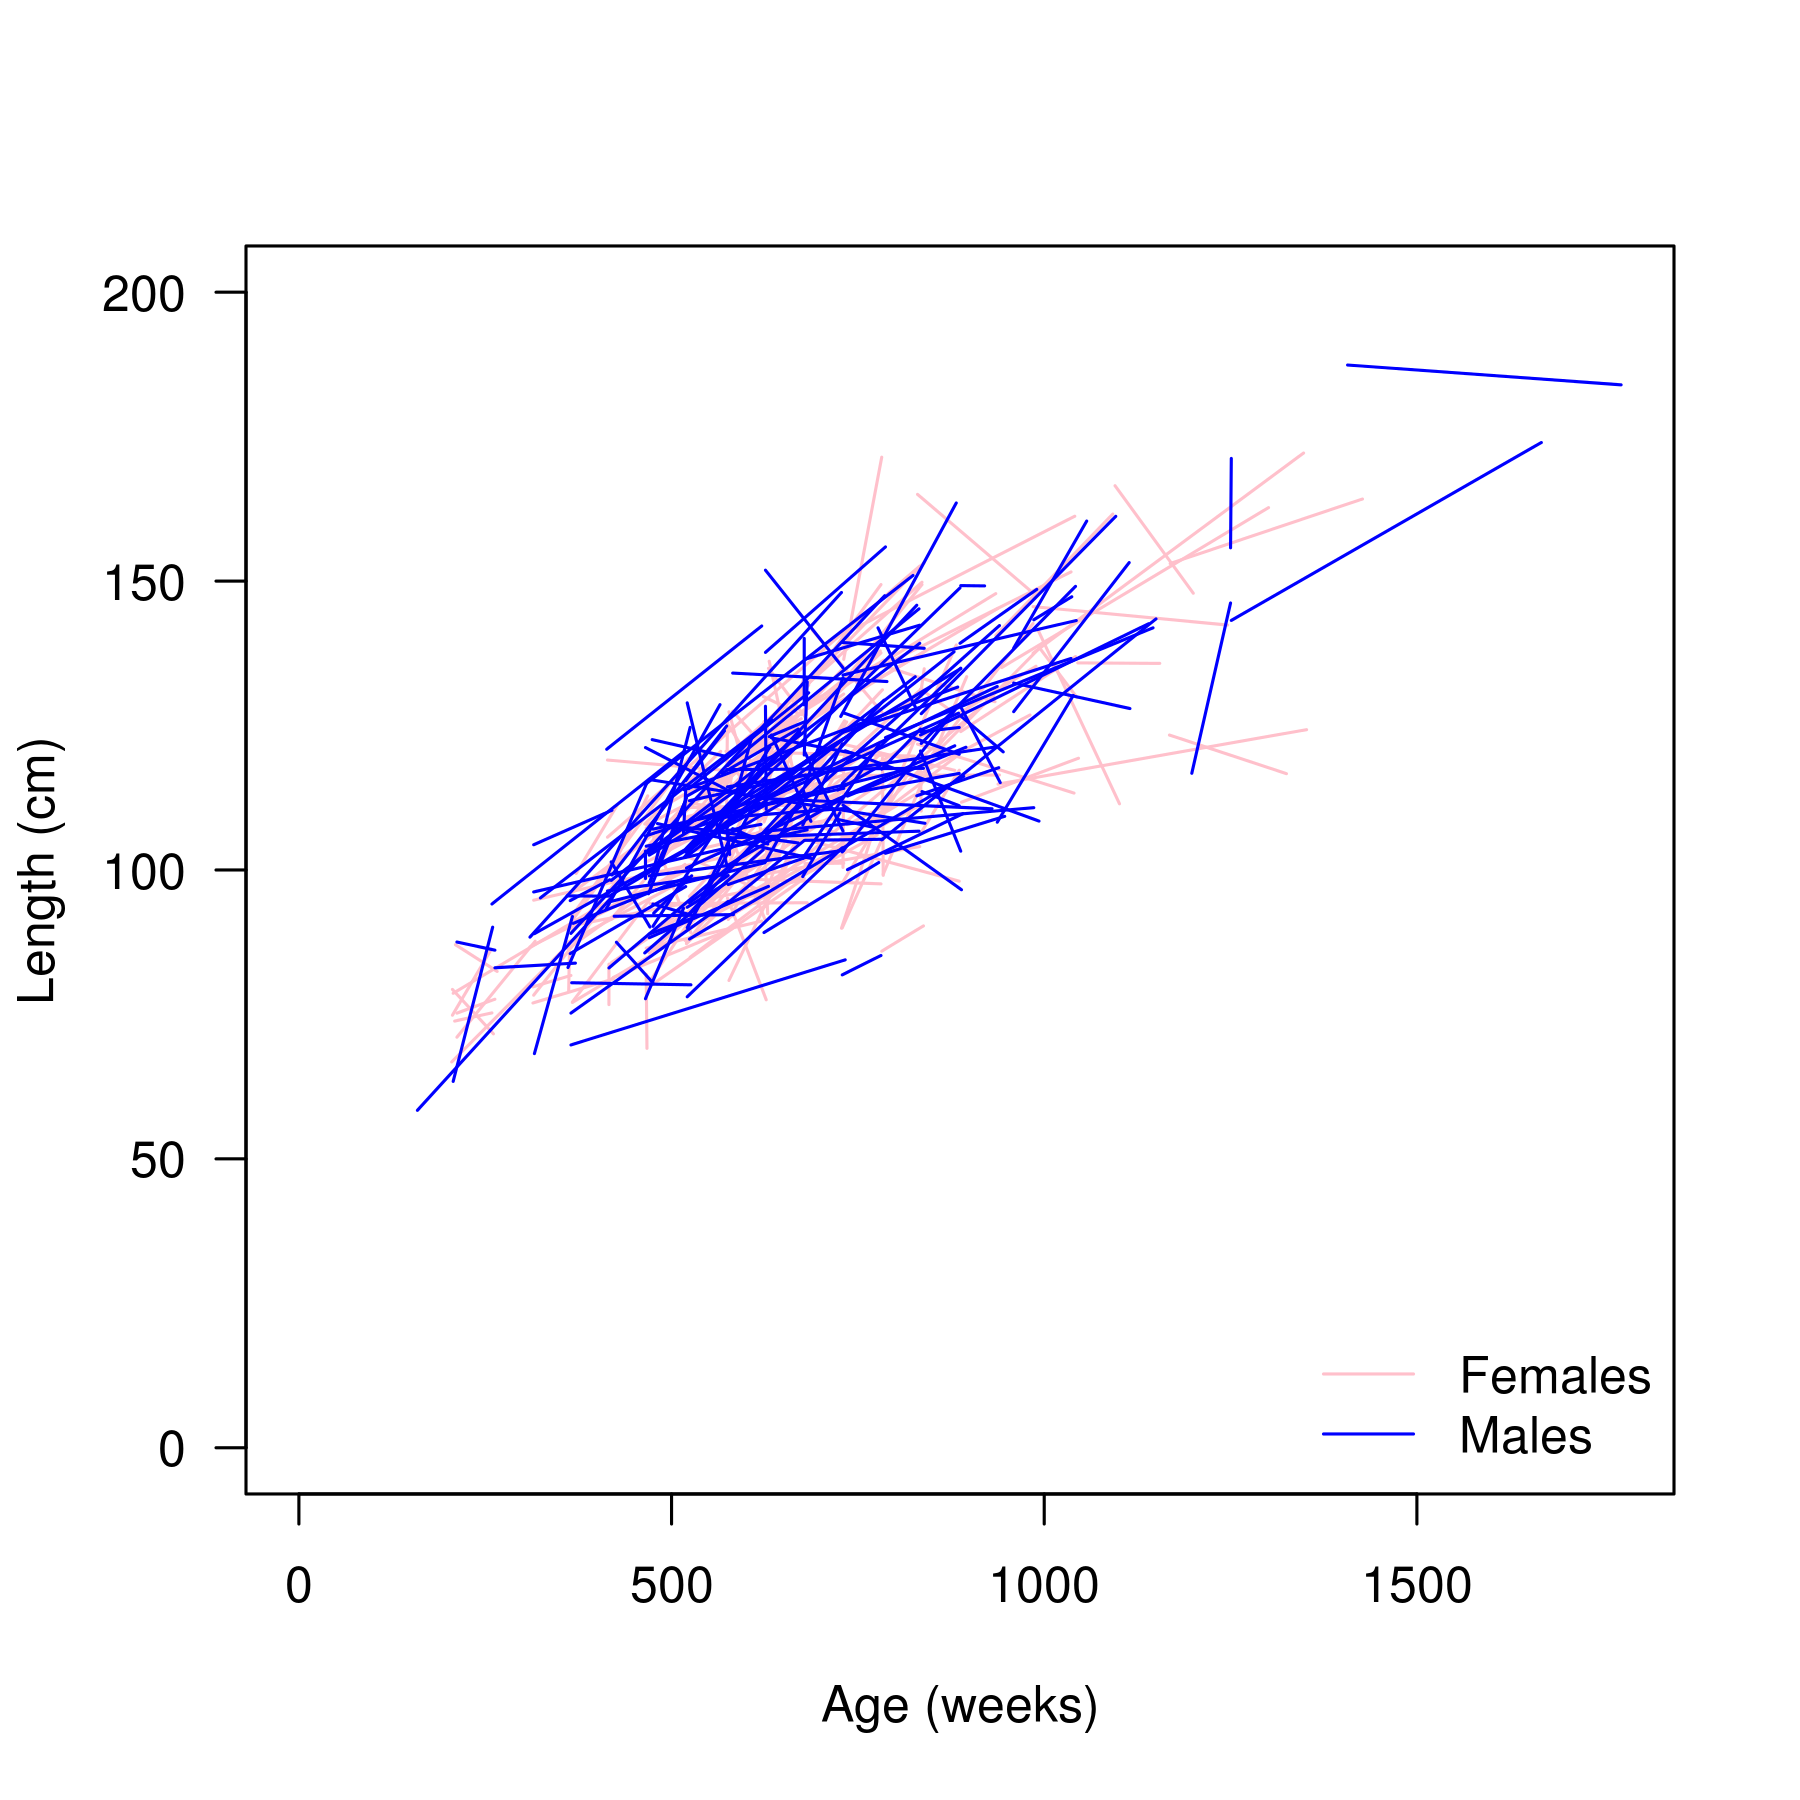
\includegraphics[width=0.49\linewidth]{../simulation/sims/growth-2.png}
  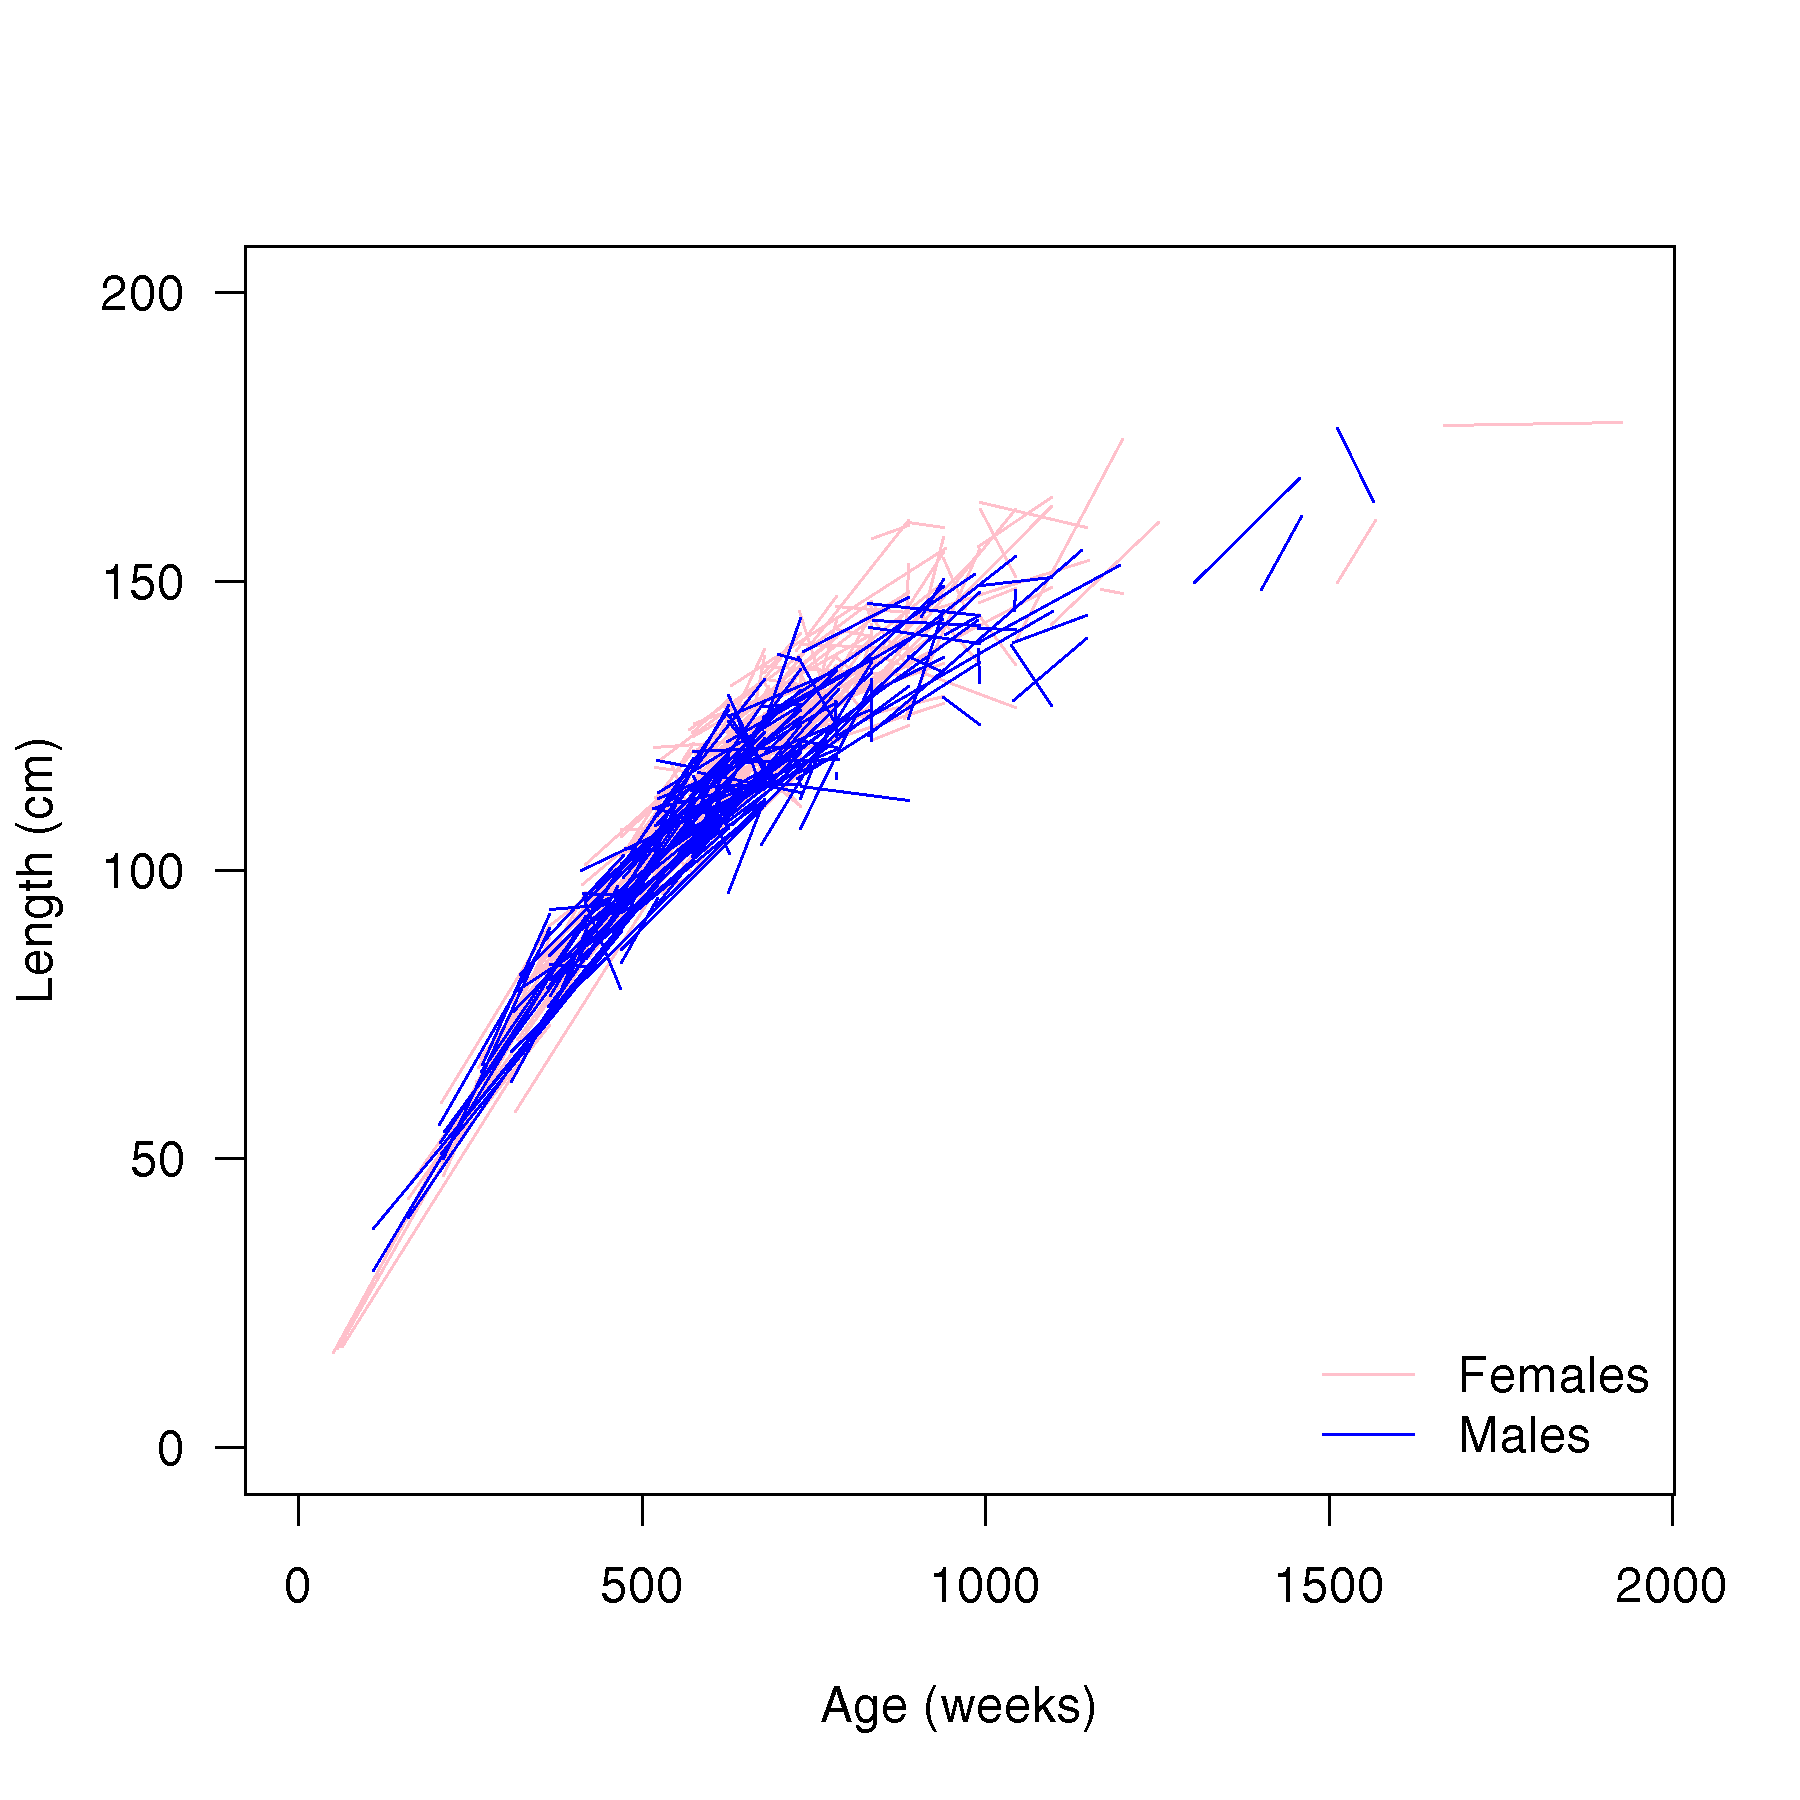
\includegraphics[width=0.49\linewidth]{../simulation/sims/growth-6.png}
  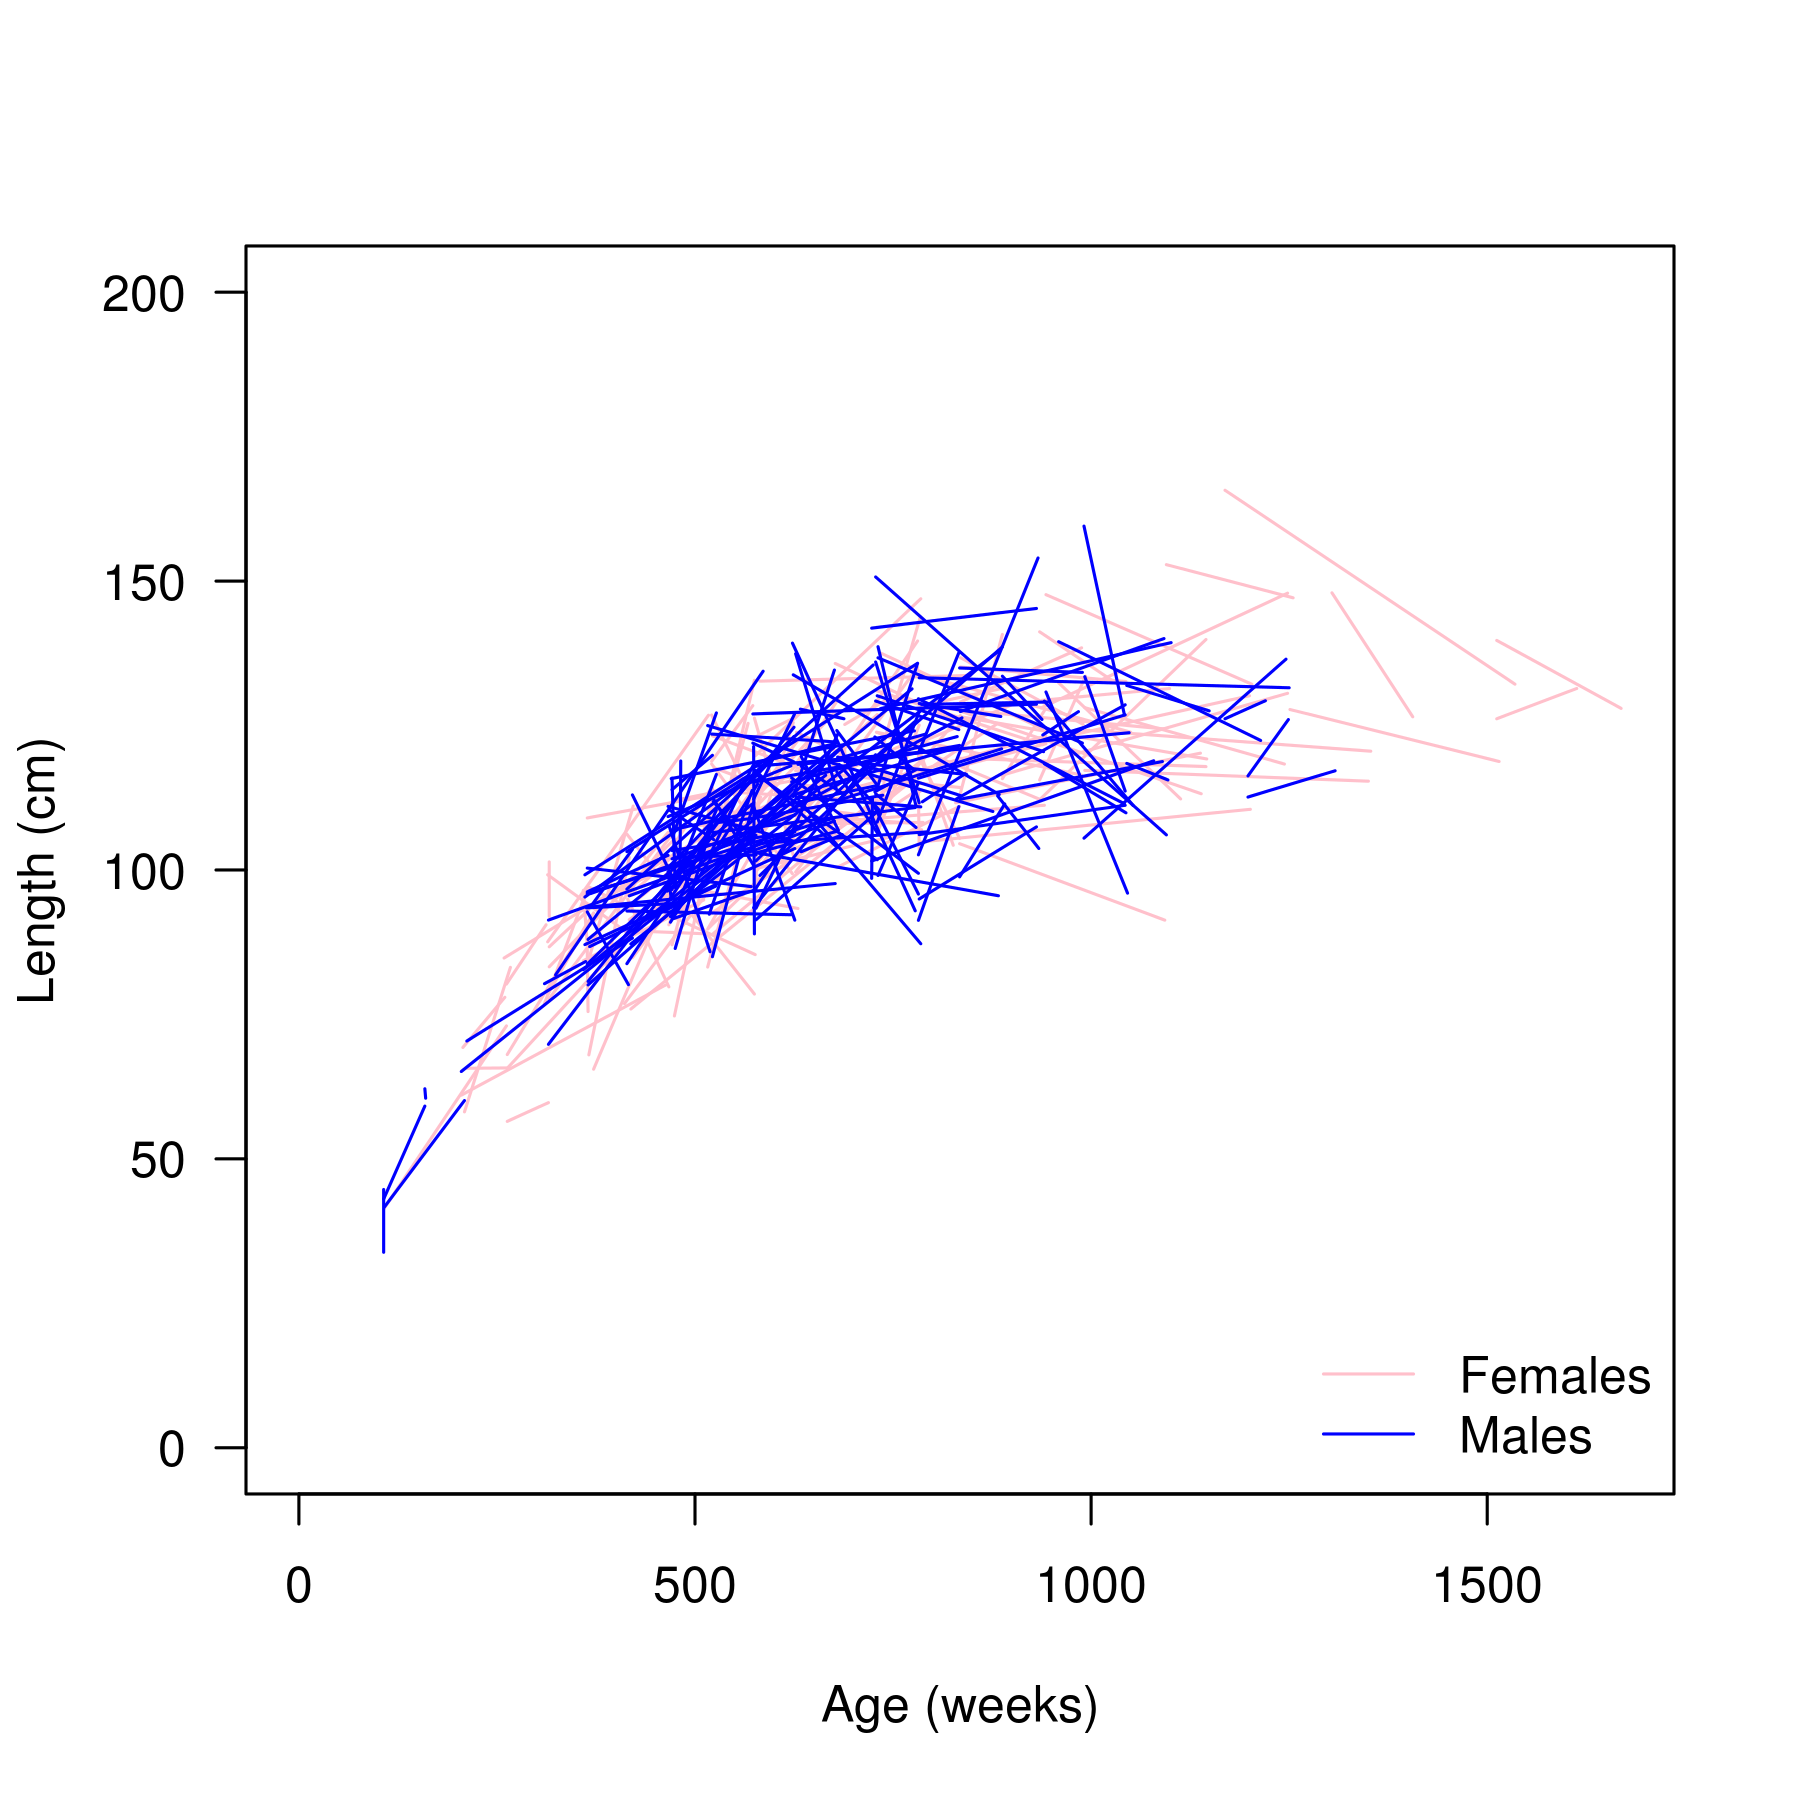
\includegraphics[width=0.49\linewidth]{../simulation/sims/growth-45.png}
  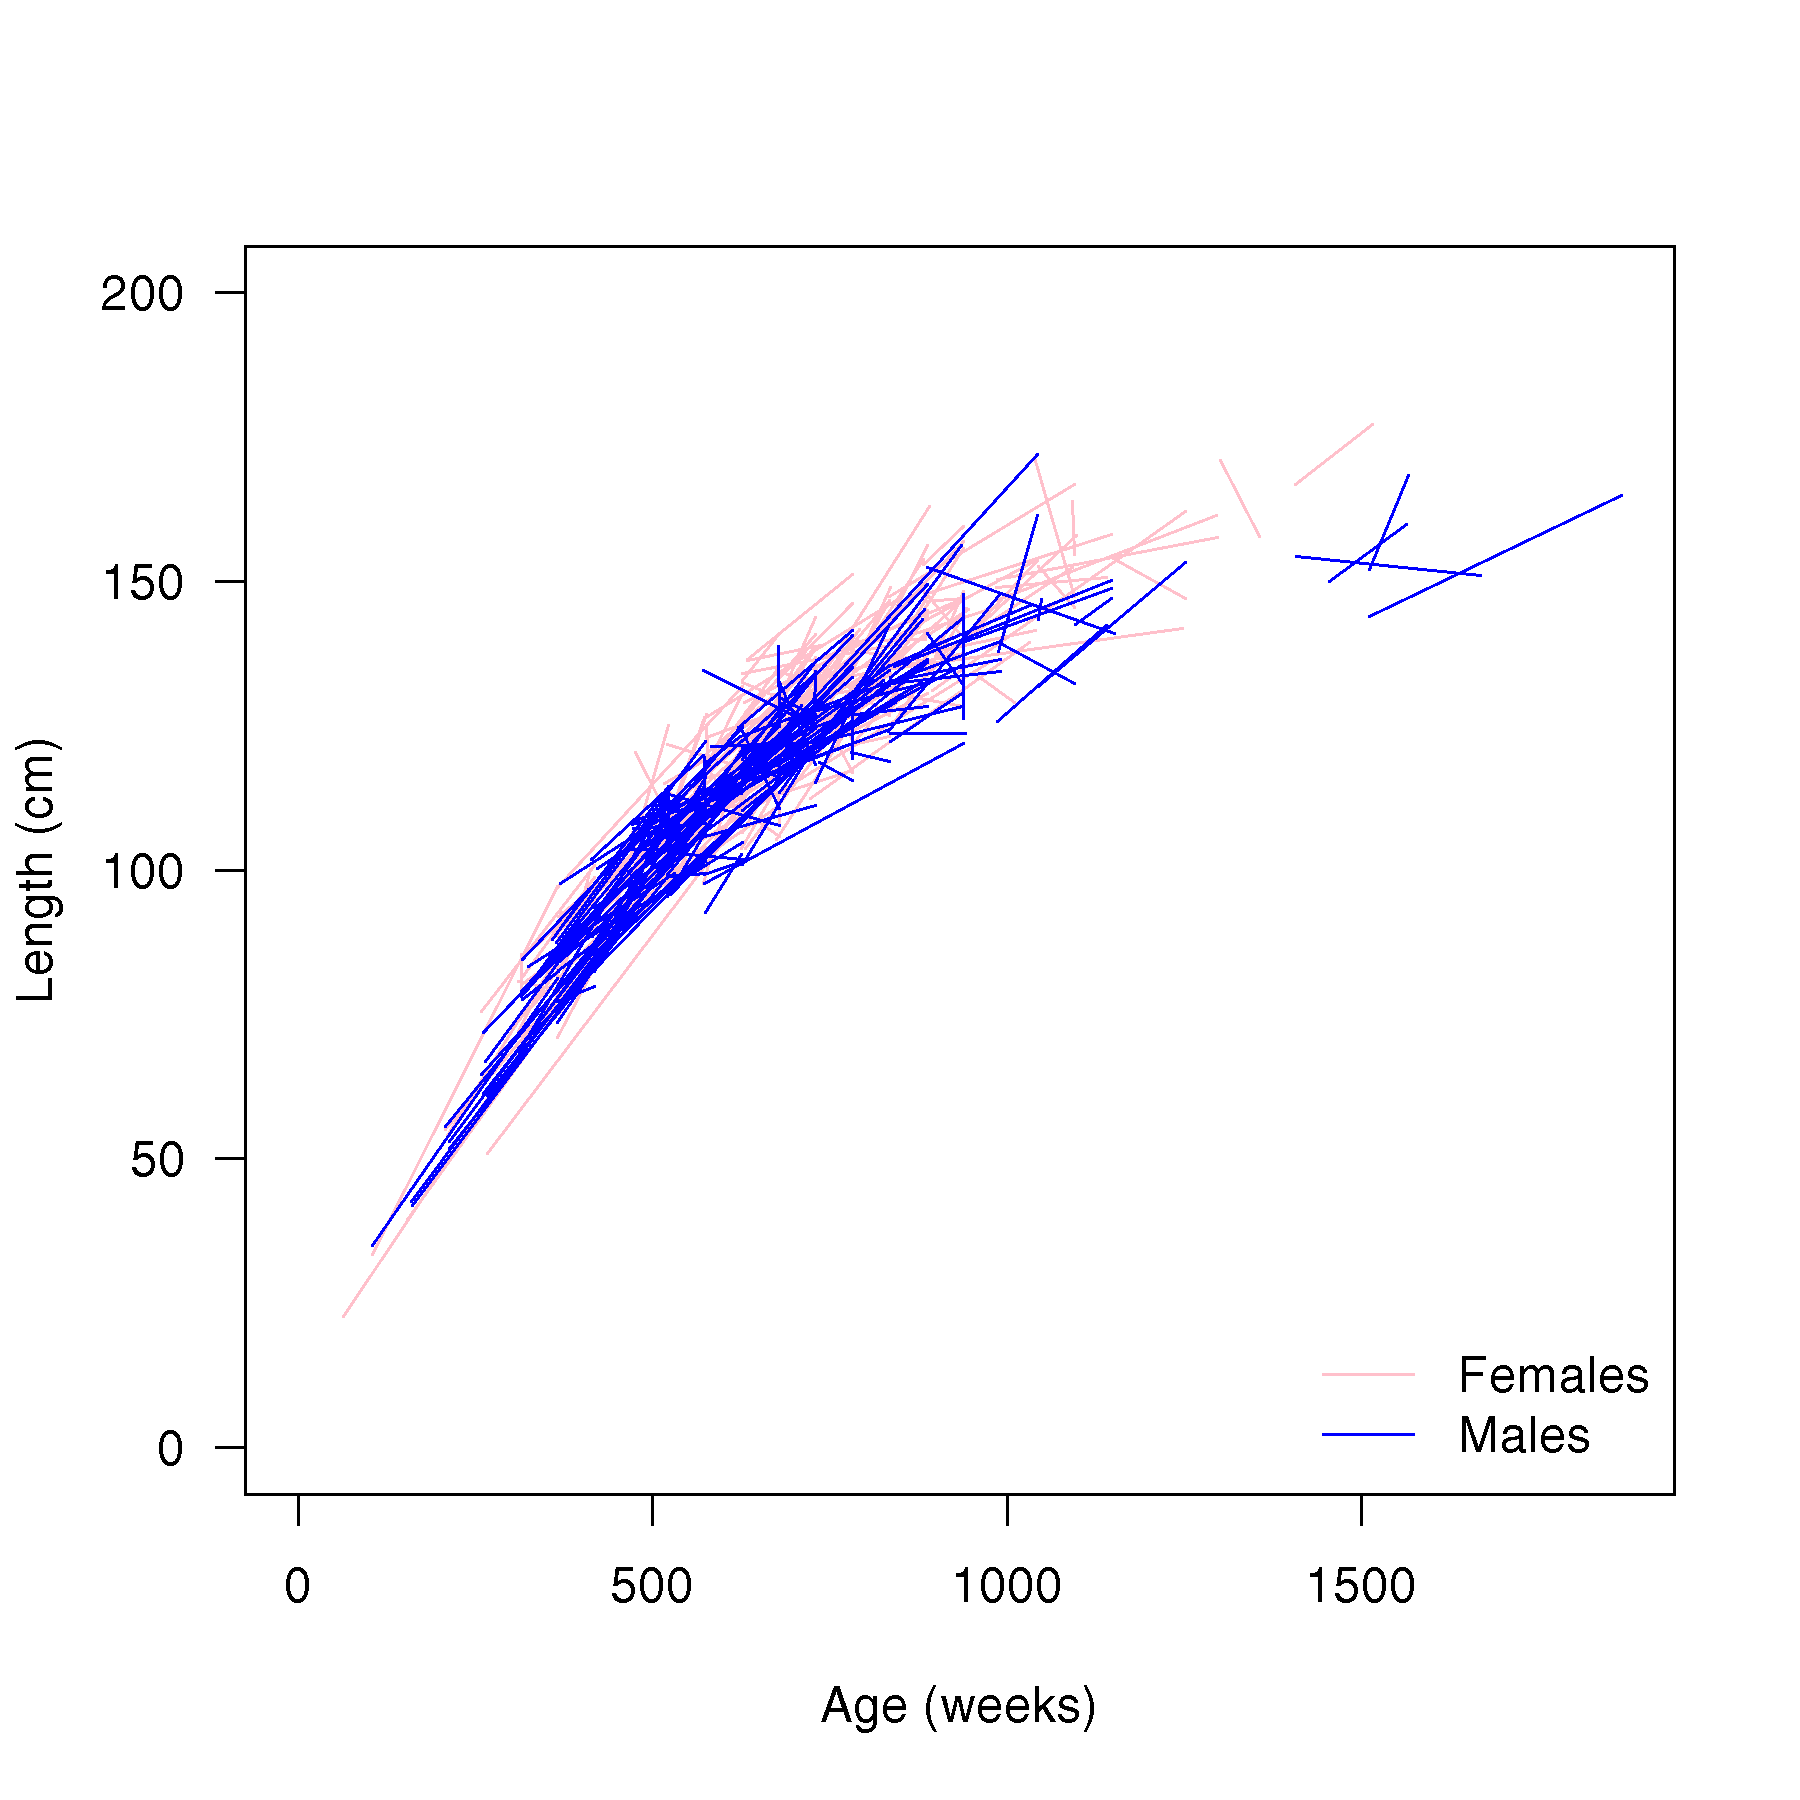
\includegraphics[width=0.49\linewidth]{../simulation/sims/growth-20.png}
  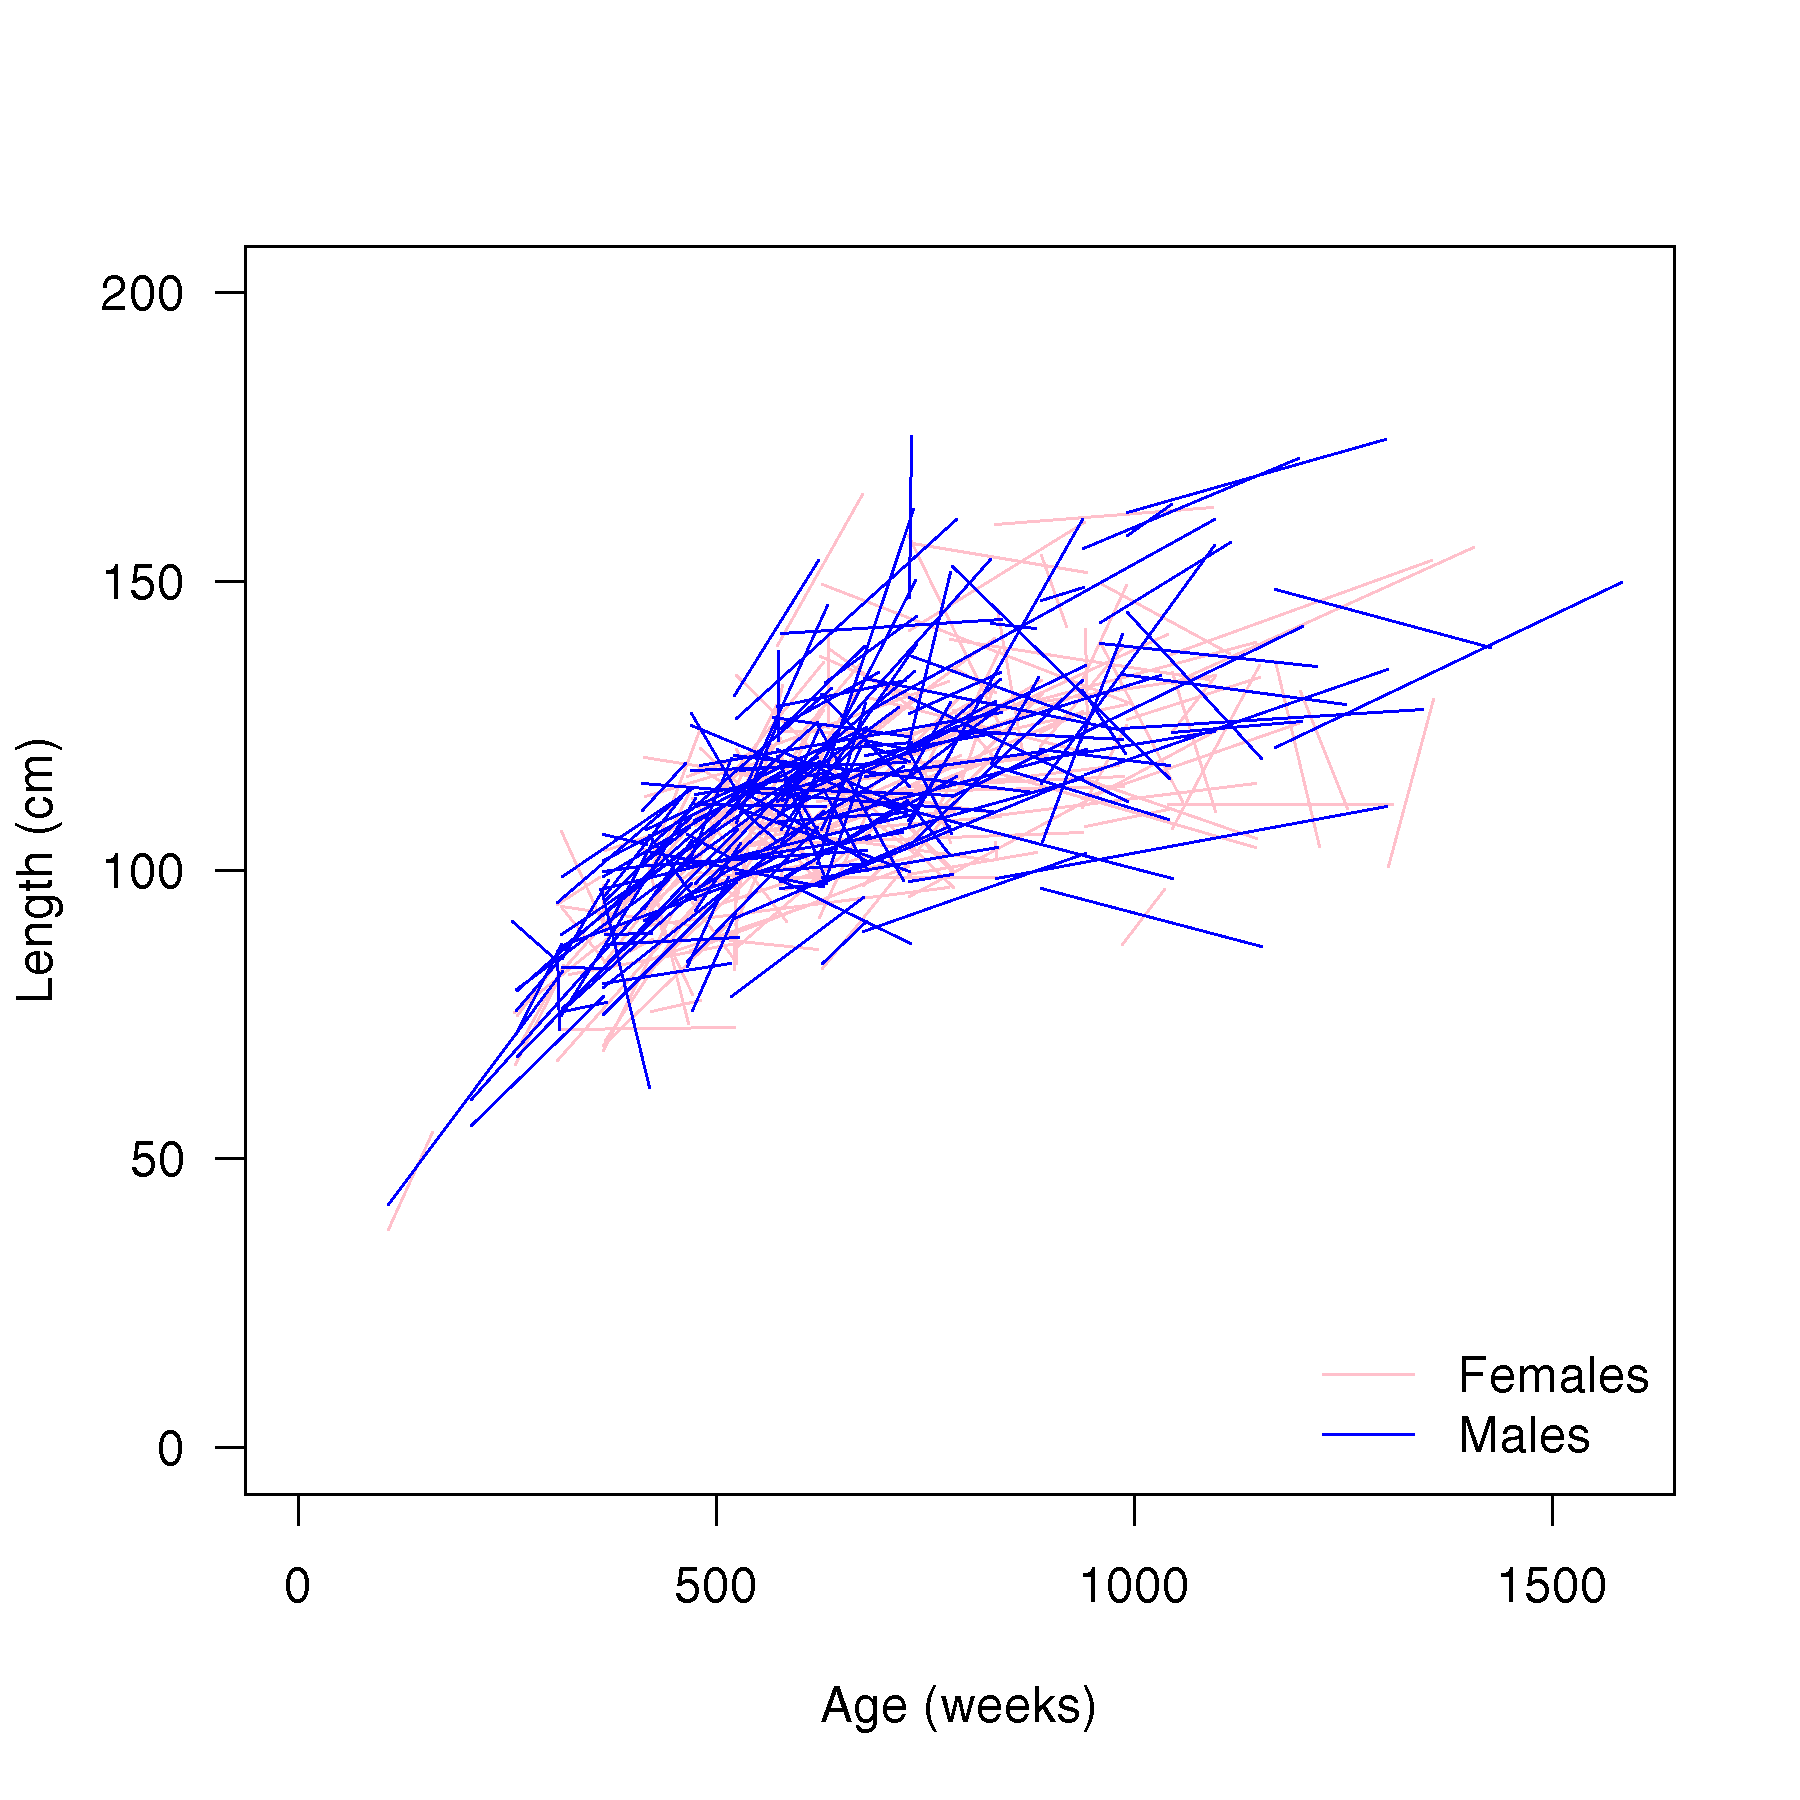
\includegraphics[width=0.49\linewidth]{../simulation/sims/growth-29.png}
  \begin{quote}
    \caption{Data sets for two models that were not pdH [top, simulations 1 and
      2], failed to converge [middle, simulations 6 and 45] and the only two
      datasets that were pdH [bottom, simulations 20 and 29].}
  \label{fig:1}
  \end{quote}
\end{figure}




%\bibliographystyle{agsm}
%\bibliography{refs/myrefs}

\end{document}

%%%%%%%%%%%%%%%%%%%%%%%%%%%%%%%%%%%%%%%%%%%%%%%%%%%%%%%%%%%%%%%%%%%%%%%%%%%%%%%%%
%%%%%%%%%%%%%%%%%%%%%%%%%%%%%%%%%%%%%%%%%%%%%%%%%%%%%%%%%%%%%%%%%%%%%%%%%%%%%%%%%
